\documentclass[openany]{book}
\usepackage[utf8]{inputenc}
\usepackage{verbatim}
\usepackage[hypertexnames=false]{hyperref}
\usepackage{amstext} 
\usepackage{array}   
\newcolumntype{C}{>{$}c<{$}} 


\input{structure}
\usepackage{geometry}
\geometry{
    top=3cm,
    bottom=3cm,
    left=3cm,
    right=3cm,
    headheight=14pt, 
    footskip=1.4cm,
    headsep=10pt,
}
\usepackage{graphicx}
\title{Apuntes de Análisis Funcional}
\author{Paco Mora}
\date{\today}

\begin{document}

\maketitle

\chapter{Yo qué sé qué es esto}

\section{Introducción}

\begin{definition}
    
    Un espacio de medida nula de primera categoría cuando está contenido en una unión numerable de cerrados con interior vacío. Si no es de primera categoría se llama de segunda categoría.
\end{definition}


\begin{theorem}
    \textbf{(Baire)}    

    Sea $ (X,d) $ espacio métrico completo $ \{G_n\}_{n \in \mathbb{N}} $ abiertos de en $ X $, $ \overline{G}_{r} = X\ \forall n \in N $. Entonces:
    $$ \bigcap_{n=1}^{\infty}G_n \ne \emptyset $$
\end{theorem}

\textit{\textbf{//Repaso de la relación de orden}}

\begin{theorem}
    \textbf{Principio de la buena ordenación }
    Para todo conjunto $ \mathcal{S}   $, existe una relación de orden $ \leq  $ tal que $ (S, \leq ) $ está bien ordenado, $ \leq  $ es un buen orden.
\end{theorem}


\begin{theorem}
    \textbf{Lema de Zorn}

    Si $ (P,\leq ) $ es un conjunto parcialmente ordenado en el que cada cadena tiene una cota superior (para $ C $, cadena, existe $ c \in P $ tal que $ x\leq c $ para todo $ x \in C $), entonces $ P $ tiene un elemento maximal (existe $  m \in P $ tal que si $ \leq x $ entonces $ x = m $)
\end{theorem}

\begin{theorem}
    \textbf{Principio Maximal de Hasudorff}

    Cada conjunto parcialmente ordenado ($ P,\leq  $) contiene una cadena maximal.

\end{theorem}

\newpage
\begin{theorem}
    Son equivalentes:
    \begin{enumerate}
        \item El principio Maximal de Hasudorff
        \item Lema de Zorn
        \item Principio de la buena ordenación
        \item Axioma de elección
    \end{enumerate}
\end{theorem}

//Definiciones de espacio de Hilbert y de Banach


//1.2.8 del libro

//Del 1.3 ha dicho que lo leamos.

//"Los teoremas que pregunto son los que tienen nombre"


\begin{theorem}
    \textbf{De la mejor aproximación}

    Dado $ (H,<\cdot >) $ espacio de Hilbert y $ C \subset H $ cerrado y convexo. Sea $ x_0 \not  \in C $. Entonces existe un único elemento $ c_0 \in C $ tal que $ \|x_0-x\| = \inf \{\|x_0-c\|\ = \alpha :\ c \in C\} $

\end{theorem}

\begin{demonstration}
    Tomemos una sucesión $(c_n)_{n \in \mathbb{N}}$ con $ c_n \in C $ de forma que se verifique 

    %imagen

    \begin{tikzpicture}
        \draw[black, very thick] (0,0) rectangle (4,0);
        \node[circle,inner sep=1pt,fill=red,label={$\alpha$}] at (1,0) {};
        \node[circle,inner sep=1pt,fill=red,label={$\|c_n\|$}] at (2,0) {};
        \node[circle,inner sep=1pt,fill=red,label={$\alpha +\dfrac{1}{n}$}] at (3,0) {};
    \end{tikzpicture}

    Si $ c_n $ fuera de Cauchy, existe $ c_0 = \lim_{n \to \infty} c_n $. Probemos que $ (c_n) $ es de Cauchy. Para ello basta usar la identidad del paralelogramo.

    Como $ \underbrace{2\|c_n\|^2}_{2 \alpha ^2}+ \underbrace{2\|c_m\|^2}_{2 \alpha ^2}-\|c_n+c_m\|^2 = \|c_n-c_m\|^2 $

    Dividimos la expresión por 4 podemos usar la convexidad de $ C $ para el punto medio entre $ c_n $ y $ c_m $:
    $$ \dfrac{1}{2}\|c_n\|^2 + \dfrac{1}{2}\|c_m\|^2 - \left\|\dfrac{c_n+c_m}{2}\right\| ^2= \dfrac{1}{4}\|c_n-c_m\|^2 $$

    Ahora tomamos límites para ver que $ \|c_n-c_m\| \to 0 $.

\end{demonstration}

\begin{theorem}
    \textbf{(de la proyección)}    

    Sea $ M  $ un subespacio cerrado del Hilbert $ H $, entonces existen un único par de aplicaciones lineales continuas $ P,Q: H \to H $ tales que $ P(H) = M $ y $ Q(H) = M^{\perp } = \{y \in H:\ <y,m> = 0\ \forall  m \in M\} $ y $ x = Px+Qx\ \forall x \in H $

    Además se verifica:
    \begin{itemize}
        \item $ x \in M \implies Px =x,\ Qx = 0;\ x \in M ^{\perp} \implies Px = 0,\ Qx = x $
        \item $ \|x-Px\| = \inf \{\|x-y\|,\ y \in M\}\ \forall x \in H $
        \item $ \|x\|^2 = \|Px\|^2+\|Qx\|^2 $ (Pitágoras)
    \end{itemize}

    Como consecuencia $ H = M \oplus M^{\perp} $
\end{theorem}

\begin{demonstration}

    Sea $ x \in H,\ x+M $ cerrado y convexo, llamemos $ Qx $ alúnico elemento en $ x+M $ de norma mínima y definimos $ Px = x-Qx $. Vemos que $ Qx \in M^{\perp} $, $ <z,y> = 0 \forall y \in M $. Aplicando que $ Qx \equiv Z $ tiene norma mínima en $ x+M $ tendremos:
    $$ 0\leq  \|z\|^2 = <z,z> \leq  \underbrace{\|z-\alpha y\|^2}_{ \forall \alpha \in \mathbb{R}} = <z-\alpha y,z-\alpha y> = \cancel{<z,z>} - \overline{\alpha}<z,y> - \alpha <y,z> = \alpha ^2\|y\|^2  $$
    
    Tomando ahora $ \alpha = <z,y>  $ y como se tiene que cumplir siempre que la expresión es mayor o igual que 0 llegamos a $ 0 \leq  -\alpha ^2 \implies \alpha = 0 $, luego $ \operatorname{Im}(Q) \subset H^{\perp} $. Como además $ M \cap M^{\perp} = \{0\} \implies x = Px+Qx $, entonces $ H = M \oplus M^{\perp} $

    Análogamente sale el resto de los enunciados\footnote{xd}.

\end{demonstration}

\begin{lemma}
    $ M \subset H $ subespacio estricto cerrado del espacio de Hilbert H. Entonces $ \exists x_0 \ne 0, x_0 \perp M $, $ <x_0,m\geq 0 \forall m \in M $

\end{lemma}
\begin{demonstration}

    Como $ H \ne M \implies M ^{\perp} \ne \{0\} $
    $$ \{d_n:\ n=1,2,..\} \text{numerable y denso en }H$$
    
    Tomamos entonces una base ortonormal $ \{e_1,e_2,...,e_n,...\} $ tal que:
    $$ \operatorname{span} \{d_1,...,d_n,...\} = \operatorname{span} \{e_1,...,e_n,...\} $$
\end{demonstration}
    
    \begin{definition}
        
        \textbf{Conjunto ortonormal} $ \{\overline{u}_1,\overline{u_2},...\} $ en $ H:\ <u_i,u_j> = \delta_{ij} $. Tenemos además que son LI:
        $$ 0 = \|\sum\limits_{i=1}^{n}c_i 0_{i}\|^2 = <\sum\limits_{i=1}^{n}c_i 0_{i},\sum\limits_{i=1}^{n}c_i 0_{i}> = \sum\limits_{i=1}^{n}c_i^2 \implies c_i = 0,\ i=1,2,...,n$$
    \end{definition}

    \begin{proposition}
        $ M = \operatorname{span} \{u_1,u_2,...,u_n\} \subset H,\ P_{M}(x) = \sum\limits_{i=1}^{n}<x_i,u_i>u_i$. Si $ d = dist \{x,M\} $ entonces:
        $$ \|x\|^2 - \delta ^2 = \sum\limits_{i=1}^{n}|<x,u_i>|^2 $$
    \end{proposition}

    \begin{lemma}
        Sea $ \{u_1,u_2,...,u_n,...\} $ ortonormal, $ \|x\|^2 \geq \sum\limits_{i=1}^{\infty} |<x,u_i>|^2\ \forall x \in H$
    \end{lemma}
\newpage
\begin{proposition}
    $ \{u_1,u_2,...,u_n,...\} $ ortonormal en $ H $, la función:
    $$ \Lambda: H \to \ell^2\ \Lambda(x) = \left( <x,u_i>   \right)_{i=1}^{\infty} $$
    es continua y sobre
\end{proposition}

\begin{demonstration}
    $ (\xi_n) \in \ell ^2 $ encontramos $ x \in H $: $ \Lambda(x) = (\xi_n) $. Nos preguntamos si:
    $$ \sum\limits_{i=1}^{\infty} \xi_nu_n \to <\sum\limits_{n=1}^{\infty}\xi_nu_n,u_m> $$

    No se ve nada en la pizarra, ha probado que es de Cauchy para ver que es convergente.

\end{demonstration}



\begin{theorem}
    \textbf{(de la base hilbertiana)}

    Para $ \{u_1,u_2,...,u_n,...\} $ conjunto ortonormal en $ H $ (espacio de Hilbert). Son equivalentes:
    \begin{enumerate}
        \item $ \{u_1,u_2,...\} $ es ortonormal maximal.\vspace{3mm}
        \item $ \overline{\operatorname{span} \{u_1,...\}} = H $
        \item $ \forall x \in H $ se tiene $ x = \sum\limits_{n=1}^{\infty}<x,u_n>u_n $ en $ H $
        \item $ \forall x \in H,\ \forall y \in H $, se tiene $ <x,y> = \sum\limits_{n=1}^{\infty}<x,u_n>\overline{<y,u_n>} $
        \item $ \forall x \in H $, se tiene $ \|x\|^2 = \sum\limits_{n=1}^{\infty}|<x,u_n>|^2 $

    \end{enumerate}
    A la igualdad de los dos últimos puntos se le llama Identidad de Parseval
\end{theorem}

\begin{demonstration}
    Recomiendo mirar el libro.
    $ 1 \iff 2 $

    Por la definición.\\
    $ 2 \implies 3 $

    Por la desigualdad de Bessel.

    Sea $ M_n = span \{u_1,u_2,...,u_n\} $, sabemos que $ \overline{\bigcup_{n=1}^{\infty}M_n} = H $ y que:
    $$ \forall x \in H,\ P_{M_n}(x) = \sum\limits_{i=1}^{n}<x,u_i>u_i $$
    $$ \|x\|^2 = \underbrace{dist(x,M_n)^2}_{=: \delta_n \to 0 } + \sum\limits_{i=1}^{n}|<x,u_i>|^2 $$
    $$ \forall\ \varepsilon >0,\ \exists x_{\varepsilon} \in \bigcup_{i=1}^{\infty} M_n:\ \|x-x_{\varepsilon}\| < \varepsilon,\ x_{\varepsilon} = \sum\limits_{i=1}^{n}c_iu_i \in M_{P} $$
    $$ \delta_{p} = d(x,M_{p}) \leq \|x-x_{\varepsilon}\| < \varepsilon $$
    $ 3 \implies 4 $\\

    Continuidad del producto escalar\\
    $ 4 \implies 5 $
    
    Directo.\\
    $ 5 \implies 2 $

    Por la desigualdad de Bessel.
\end{demonstration}

\begin{definition}
    A una base como la anterior se le llama \textbf{base hilbertiana}. A los coeficientes se les llama coeficientes de Fourier.
\end{definition}

\begin{lemma}
    Si $ (E,\|\cdot \|) $ es un espacio de Banach con una base algebraica numerable, entonces $ E $ es finito dimensional. 
    
    Para $ E $ no completo, no es cierto.
\end{lemma}

Aquí falta un teorema que ha dictado y no me ha dado tiempo a copiar.

% Teorema que se acaba de inventar
% Dado u producto escalar en el pro
% El coeficiente del termino de grado $n$ en $phi_{n}$ puede tomarse siempre positivo y si asi se hace la sucesión $phi_{n}$ esta unívocamente determinada.

\begin{theorem}
    Sea $ <\cdot > $ un producto escalar en $ C([a,b]) $ con $ \|\cdot \|_{\infty} $ más fina que $ \|\cdot \|_{\infty} $. Sea $ \{\phi_{n}: n = 0,1,2,\dots\}  $ la sucesión de polinomios ortonormales. Entonces:
    $$ f = \sum\limits_{n=0}^{\infty}<f,\phi_n>\phi_n\ \forall f \in C[a,b] $$

    $$ \forall \varepsilon>0\ \exists N_{\varepsilon} \implies \left\|f - \sum\limits_{n=0}^{\infty}<f,\phi_{n}>\phi_n\right\|_{<\cdot >} < \varepsilon$$
\end{theorem}


\subsection{Series de Fourier}

\begin{definition}
    Un polinomio trigonométrico es una función de la forma
    $$ h(t) = \sum\limits_{n=0}^{m} \alpha_n \cos(nt)+\beta_n \sin(nt),\ \alpha_n,\beta_n \in \mathbb{R},\ m = 0,1,2,... $$

\end{definition}

\begin{lemma}
    Si $ h_1,h_2 $ son polinomios trigonométricos, su producto también lo es.
\end{lemma}

\begin{lemma}
    $ f: [- \pi, \pi] \to \mathbb{R},\ \varepsilon>0 $, entonces existe un polinomio trigonométrico $ q_{\varepsilon} $ tal que:
    $$ \int\limits_{-\pi}^{\pi}|f(t)-q_{\varepsilon}(t)|^2 dt < \varepsilon $$
\end{lemma}

\begin{exercise}
    $$ u_0(t) = \dfrac{1}{\sqrt{2\pi}},\ u_{2n+1}(t) = \dfrac{1}{\sqrt{pi}} \cos(nt),\ u_{2m}(t) = \dfrac{1}{\sqrt{pi}} \sin(mt),\ m = 1,2,... $$
    Es ortonormal en $ (C[a,b],\langle\cdot \rangle) $
\end{exercise}


\section{Teoremas de representación}

Vemos primero un primer teorema de representación.

\begin{proposition}
    Dado $ F:C[0,1]\to \mathbb{R} $  lineal y continua. Existe una única medida ($ F $ función de distribución) tal que:
    $$ F(f) = \int\limits_{0}^{1}f(t)dF(f) $$
\end{proposition}

%teorema de alexandrov ???

%topología debil

\begin{theorem}
    \textbf{Teorema de Riesz}.

    Buscar en el libro.
\end{theorem}


\begin{definition}\textbf{Topología débil del espacio de Hilbert}

    Sea $ (H,<>) $ un espacio de Hilbert. 
    $$ 
    \begin{aligned}
        \mathbb{K} \leftarrow H : x_0, & \hspace{10mm} \varepsilon>0,\  t_1,...,t_p \in H\\ <x,x_0> \hookleftarrow x
    \end{aligned}
    $$
    $$ W(x_0,\varepsilon,t_1,...,t_p) = \{z \in H: |<t;x_0-z>|< \varepsilon,\ i=1,2,...,p\} $$
\end{definition}

\begin{theorem}
    \textbf{Alaoglo-Bourbaki}

    Sea $ (H,<>) $ un espacio de Hilbert y sea $ B_{H} = \{x \in H:\ \|x\|_{<>} \leq  1\} $. Entonces $ B_{H} $ es un subconjunto débilmente compacto.
\end{theorem}


%teoremas necesarios para esto, teorema de skolin (la topo de la puntual y puntual sobre un denso conincide)
%2 t skolin (tambien coincide sobre idk)

\begin{demonstration}

    Lo vemos para el caso separable.

    Tomemos una base hilbertiana $ \{e_n\} $ de $ H $ y tomemos $ (v_n) \subseteq  B_{H} $.
    
    Notemos primero que $ |<e_{p},v_n>| \leq  1\ \forall p,n \in \mathbb{N} $. 

    Tomemos $ [0,1]^{\mathbb{N}} $, el cubo de Hilbert, que es métrico compacto.

    Por el teorema de Riesz, tomamos la forma lineal equivalente a cada elemento de la sucesión $ (v_n) $, $ v_n \mapsto <-,v_n > $ y utilizando la base, este producto puede expresarse como $ \sum\limits_{p=1}^{\infty} <x,e_{p}>e_{p} $ para cierto $ x $.

    Volviendo al cubo de Hilbert, existe una sucesión de enteros $ n_1<n_2,...,n_{k}<... $ de forma que $ (<e_{p},v_{n_{k}})_{k=1}^{\infty} $ es convergente (ya que el cubo es métrico compacto).

    Si tomamos entonces $ S = s\operatorname{span}\{e_n:\ n \in \mathbb{N}\} $, entonces $ (<s,v_{n_{k}}>)_{k=1}^{\infty} $ es convergente $ \forall  s \in S $. Falta ver que sea convergente para todo punto de $ H = \overline{S} $ que se demuestra con los teoremas de Skald que se ven a continuación.

\end{demonstration}

\section{Familias de funciones equicontinuas}

\begin{definition}
    \textbf{Familia de funciones (uniformemente) equicontinua}

    Una sucesión de funciones continuas $ (f_{i})_{i \in I} $ se dice que es equicontinua en $ x_0 $ si $ \forall  \varepsilon > 0\ \forall i \in I\  \exists \delta_{\varepsilon}$ tal que $ d(x_0,x) < \delta_{\varepsilon} \implies |f_{i}(x)-f_{i}(x_0)| < \varepsilon $. Es decir, que el $ \delta  $ necesario es el mismo para todas las funciones.
    
    De forma análoga se define el concepto de familia de funciones uniformemente equicontinua:
    
    Una sucesión de funciones uniformemente continuas $ (f_{i})_{i \in I} $ se dice que es uniformemente equicontinua en si $ \forall  \varepsilon > 0\ \forall i \in I\  \exists \delta_{\varepsilon}$ tal que $ d(y,x) < \delta_{\varepsilon} \implies |f_{i}(x)-f_{i}(y)| < \varepsilon $. Es decir, que el $ \delta  $ necesario es el mismo para todas las funciones.
\end{definition}

Las demostraciones de los teoremas se pueden encontrar en el libro General Topology de Willard (va para tarea).

\begin{theorem}
    Sea $ (K,d) $ un espacio métrico y $ \operatorname{C}(K) = \{f: K \to \mathbb{R}\ \text{continuas}\} \hookrightarrow (\mathbb{R}^{k},T_{p}) $ ($ T_{p} $ es la topología producto). 

    Si $ \phi $ es (unif.) equicontinua, entonces $ \overline{\phi}^{T_{p}}  $ son (uniformemente) continuas
\end{theorem}

\begin{theorem}
    Si $ \phi $ es equicontinua, entonces en $ \phi $ coinciden las topologías $ T_{p} $(producto) y la de convergencia puntual sobre un subconjunto $ D \subseteq K $ denso ($ \overline{D} = K $).
\end{theorem}


\begin{theorem}\textbf{De Ascoli}

    Sea $ \phi \subseteq  \operatorname{C}(K)$ y sea $ (K,d) $ métrico compacto. Entonces $ \phi $ es relativamente compacto en $ \|\cdot \|_{\infty} \iff \phi  $ es equicontinuo y $ \phi(x) = \{f(x): f \in \phi\} $ acotado $ \forall x \in K $
\end{theorem}


%Otra tarea que no me entero del enunciado: Diestel Spaces and Sequences in Banach spaces

\begin{theorem}\textbf{Lax- Milgram}


    Sea $ (H,<>) $ un espacio de Hilbert y $ B: H \times H \to \mathbb{K} (\mathbb{R}\ o\ \mathbb{C}) $ tal que:

    \begin{enumerate}
        \item $ B(\cdot ,y) $ es lineal $ \forall y \in H $ y $ B(x,\cdot ) $ es lineal conj., es decir, $ B $ es sesquilineal.
        \item $ B $es acotada: $ \exists c > 0 $ tal que $ |B(x,y)| \leq  C \|x\|\|y\| \forall x,y \in H $
        \item $ B $ es fuertemente positiva: $ \exists b > 0 $ tal que $ |B(x,y)| > b\|y\|^2 $, $ \forall  y \in H $
    \end{enumerate}

    Entonces para cualquier forma lineal y continua $ \phi: H \to \mathbb{K} $ existe un único $ y \in H $ tal que $ \phi(x) = B(x,y)  \forall x \in H$
\end{theorem}



\begin{demonstration}
    
    Para $ y  $ fijo la apliación $ x \hookrightarrow B(x,y) $ es lineal continuo. Por el teorema de Riesz, $ \exists z \in H $ tal que $ B(x,y) = <x,z> \forall x \in H $ y sea $ T $ la forma lineal que da el teorema de Riesz. 

    Tenemos que $ T(H) $ es un subespacio de $ H $. Veamos que $ T(H) = H $ y esto dará la prueba de nuevo por el teorema de Riesz. Demostremos varias cosas:

    \begin{enumerate}
        \item $ T(H) $ es cerrado.
            $$\text{Sea } z_n = Ty_n\ \text{tal que}\ \lim_{n \to \infty} z_n = z \in H, z \in T(H) $$

            $$ B(x,y_n-y_m) = <x,z_n-z_m> \forall x \in H $$
            $$ b\|y_n-y_m\|^{\cancel{2}} \leq  B(y_n-y_m,y_n-y_m) = <y_n-y_m,z_n-z_m>\leq \cancel{ \|y_n-y_m\|} \|z_n -z_m\| $$

            Luego $ (y_n) $ es de Cacuhy y $ \lim_{n \to \infty}y_n = y $ y tenemos que:
            $$ <x,z_n>  = B(x,y_n) \to B(x,y) = <x,z> = <x,Ty> \forall x \in H $$

        \item Supongamos $ T(H) \subsetneq H \implies \exists x_0 \ne 0:\ <x_0,z> = 0 \forall z \in T(H) \implies B(x_0,y) = <x_0,z> \forall y \in H,\ B(x_0,x_0) = 0 $ si $ x_0 \ne 0 $
    \end{enumerate}

    
\end{demonstration}

\section{Principio de Dirichlet}

\noindent Para esta sección consideraremos $ \Omega $ un subconjunto de $ \mathbb{R}^{n} $ abierto y acotado.

Lo que querremos estudiar en esta sección será el siguiente sistema llamado problema de Dirichlet:

$$ \left\{
\begin{array}{ll}
    \triangle u(x) = 0 & x \in \Omega\\
    u|_{\partial \Omega}(x) = f(x) & x \in \partial \Omega 
\end{array}
\right. $$

\begin{example}
    Tomemos $ n = 2 $, en esta dimensión existe el problema clásico de una placa que se calienta en los bordes. Queremos conocer el estado estacionario del sistema.
\end{example}

\begin{flushright}
    \textbf{Idea para buscar una solución}
\end{flushright}

Buscar el estado de equilibrio minimizando una energía o acción adecuada.

La energía que plantea Dirichlet es la de la llamada integral de Dirichlet:
$$ D(u) = \int\limits_{\Omega}^{}|\triangledown u | ^2 = \int\limits_{\Omega}^{} | \dfrac{\partial u}{\partial x_1}|^2 + | \dfrac{\partial u}{\partial x_2}|^2 d_1dx_2 $$

\begin{definition}
    $ C^2(\overline{\Omega}) $

    Denotamos a $ C^2(\overline{\Omega}) $ como las funciones dos veces derivables en el interior de $ \Omega $ con segunda derivada continua en $ \overline{\Omega} $.

    Las funciones con las que trabajaremos en este apartado son las de este tipo con soporte compacto, y al conjunto de ellas las denotaremos por $ C_0^2(\overline{\Omega }) $.
\end{definition}

Para ver una proposición necesitamos repasar el siguiente teorema:

% \begin{theorem}
%     \textbf{Integración por partes en $  \mathbb{R}^{n}$}

%     Se da la igualdad:

%     $$ \int\limits_{\Omega}^{} (\partial x_j u)vdx = - \int\limits_{\Omega}^{} u (\partial x_j v)dx + \int\limits_{\partial \Omega }^{}uvn_j d \theta $$
% \end{theorem}

% \newpage
% Este teorema se generaliza en el siguiente:

\begin{theorem}
    \textbf{Teorema de Gauss}

    Dada $ \Omega  $ suficientemente regular:

    $$ \int\limits_{\Omega }^{} \partial x_j wdx = \int\limits_{\Omega }^{} w n_j d \theta $$
\end{theorem}

\begin{proposition}
    Si existe $ u \in C^2(\overline{\Omega}) $ que minimiza a $ D(u) $ entre todas las funciones $ u \in C^2(\overline{\Omega})   $ con $ u|_{\partial\Omega} \equiv f $, entonces $ u $ es armónica ($ \triangle u = 0 $).

\end{proposition}

\begin{demonstration}
    
    En $ C^2(\overline{\Omega}) $, definimos $ \<\cdot \>_{D} $ por:
    $$ \<F,G\>_{D} = \int\limits_{\Omega}^{} \left( \dfrac{\partial F}{\partial x_1} \dfrac{\partial G}{\partial x_1} + \dfrac{\partial F}{\partial x_2} \dfrac{\partial G}{\partial x_2} \right) dx_1dx_2$$

    Definimos ahora $ D(u) = \<u,u\>_{D} $.

    Si $ v \in C^2(\overline{\Omega}) $ que verifica que $ v|_{\partial \Omega} = 0 \implies \forall  \varepsilon \in \mathbb{R} $ se tiene que $ D(u+ \varepsilon v) (*)\geq  D(u) $
    $$ (*) = D(u)+ \varepsilon^2 D(u) + \varepsilon D(v) + \varepsilon \<u,v\>_{D}+ \varepsilon \<v,u\>_{D} $$

    Cancelando $ D(u) $ tenemos:
    $$ \varepsilon^2 D(u) + \varepsilon D(v) + \varepsilon \<u,v\>_{D}+ \varepsilon \<v,u\>_{D}\geq  0 $$

    Como esto lo podemos hacer para un $ \varepsilon $ arbitrario, tenemos que $ \<u,v\>_{D} = 0\ \forall v \in C^2(\overline{\Omega }) $ con soporte compacto, luego:
    $$ 0 = \int\limits_{\Omega}^{} \left( \dfrac{\partial u}{\partial x_1} \dfrac{\partial v}{\partial x_1}+ \dfrac{\partial u}{\partial x_2} \dfrac{\partial v}{\partial x_2} \right) dx_1 dx_2 $$

    Utilizando el teorema de Gauss llegaremos al resultado deseado.

    $$ \int\limits_{\Omega}^{} \left( \dfrac{\partial u}{\partial x_1} \dfrac{\partial v}{\partial x_1}+ \dfrac{\partial u}{\partial x_2} \dfrac{\partial v}{\partial x_2} \right) dx_1 dx_2 = - \int\limits_{\Omega }^{} (\triangle u)v \hspace{2mm} \forall  v \in C_0^2(\overline{\Omega })\ con\ v|_{\partial \Omega } = 0 $$

    También sabemos que $ C_0^{\infty}(\overline{\Omega }) $ es denso en $ L^2(\Omega ) $. Entonces $ \langle \triangle u, v \rangle_{L^2} = 0 $ para cualquier $ v $ de un denso, luego $ \triangle u = 0 $


\end{demonstration}

% \subsection{Estudio del espacio $ C^{1}(\overline{\Omega }) $}

% Recordemos que tenemos:

% $$ \langle u, v \rangle_{D} = \int\limits_{\Omega }^{} (\triangledown u \cdot  \triangledown v)dx \hspace{5mm} \triangledown u \cdot  \triangledown v = \sum\limits_{j=1}^{N} \dfrac{\partial u}{\partial x_j} \dfrac{\partial v}{\partial x_j} $$

% $$ \|u\|_{D}^2 = \langle u, u \rangle_{D} = \|\triangledown u\|^2_{L^2(\Omega )} $$



\begin{theorem}
    \textbf{Desigualdad de Poincaré}

    $ \forall  f \in \mathcal{D}(\Omega ) =  C_{0}^{\infty}(\Omega ) $, $ \|f\|_{0}\leq \operatorname{diam}(\Omega )\|f\|_{1} $
\end{theorem}

Como consecuencia, tenemos continuidad en la inclusión:
$$ (\mathcal{D}(\Omega ), \langle ,  \rangle_{1}) \hookrightarrow (\mathcal{D}(\Omega ),\langle ,  \rangle_{0}) $$ 

Aquí faltan varias definiciones de tipos de espacios de Hilbert. Creo que están en el libro.

\begin{lemma}$  $

    \begin{enumerate}
        \item $ H_{1}^{0} \subseteq  H_0 $
        \item $ \forall v \in H_1^{0},\ \exists v_j \in H_0: \langle z, v_j \rangle_{0} = - \langle \dfrac{\partial z}{\partial x_j}, v \rangle_{0} $. Es decir:
        $$ \int\limits_{\Omega }^{} zv_j = - \int\limits_{\Omega }^{} \dfrac{\partial z}{\partial x_j}v $$
        \item Si $ u,v \in H^{0}_{1} \implies \langle u, v \rangle_{1} = \int\limits_{\Omega }^{} \sum\limits_{j=1}^{N} \dfrac{\partial n}{\partial x_j} \dfrac{\partial v}{\partial x_j} $
    \end{enumerate}

    A $ v_j $ se le llama $ \dfrac{\partial v}{\partial x_j} $
\end{lemma}

\begin{demonstration}
    Sea $ (v_n) \in \mathcal{D}(\Omega ),\ v_n \to v \in H_1^{0} $ en $ \|\cdot \|_{1} \implies \left( \dfrac{\partial v_n}{\partial x_j} \right)_{n=1}^{\infty} $ es de Cauchy en $ \langle ,  \rangle_{0} $ y converge a una función a la que llamamos $ v_j \in H_0 = L^2(\Omega )$. Por la desigualdad de Poincaré, $ (v_n)$ es de Cauchy en $ \|\cdot \|_{0}$ y su límite no podrá ser otro que $ v$. La fórmula:
    $$ \int\limits_{\Omega }^{}zv_j = - \int\limits_{\Omega }^{} \dfrac{\partial z}{\partial x_j} v $$

    Viene dada por el paso al límite de la expresión dada por el teorema de Gauss:
    $$ \int\limits_{\Omega }^{} z \dfrac{\partial v_n}{\partial x_j} = - \int\limits_{z}^{x_j}v_n $$
    
\end{demonstration}

\begin{lemma}
    \textbf{Variacional}

    $ \Omega  \subseteq  \mathbb{R}^{n}$ abierto y acotado, $ u \in L^2(\Omega )$:
    $$ \int\limits_{\Omega }^{} uv dx = 0 \forall  v \in \mathcal{D}(\Omega )$$

    Entonces $ u = 0 $ en $ L^2(\Omega )$ y $ u = 0\ \forall  x \in \Omega $ 
\end{lemma}


\begin{theorem}
    $ $
    
    Sea $ \Omega  \subseteq  \mathbb{R}^{N}$ un abierto y acotado. Sea $ f \in L^2(\Omega ) \equiv H_0$. Entonces existe una \textbf{solución débil} de la ecuación:
    $$ \left\{
    \begin{array}{l}
        \triangle u = f\\ 
        u|_{\partial \Omega } u = 0
    \end{array}
    \right. $$ 

    En el siguiente sentido:

    {\color{red}Existe una única función $ v \in H^{0}_{1}$ donde que $ \langle u, f \rangle = - \langle u, \triangle v \rangle$ $ \forall u \in \mathcal{D}(\Omega )$}

    Lo rojo aún ''está por aclarar''
\end{theorem}


\begin{demonstration}
    Si $ f \in L^2 \implies \phi: L^2 \to \mathbb{R}$ lineal y continua en $ H_0$ por Riesz. Aplicando la des. de Poincaré:
    $$ |\phi(n)| \leq  \|f\|_{0}\|u\|_{0} \leq  \operatorname{diam}(\Omega ) \|f\|_{0}\|u\|_{1}\ \forall  u \in \mathcal{D}(\Omega ) \implies \phi \text{ es continua en } (\mathcal{D}(\Omega ),\langle ,  \rangle_{1}) $$

    Entonces podemos extender $ \phi$ al completado, $ H_1^{0}$. A esta forma lineal extendida le aplicamos el teorema de Riesz.

    Existirá entonces una única $ v \in H_{1}^{0}$ tal que $ \phi(u) = \langle u, v \rangle_{1}  = \sum\limits_{j=1}^{N} \langle u_j, v_j \rangle_{0}$ para todo $ u \in H_1^{0}$.

    Si tomamos $ u \in \mathcal{D}(\Omega )$:
    $$ \langle u, v \rangle_{1} = \sum\limits_{j=1}^{N} \langle u_j, v_j \rangle_{0} = \sum\limits_{j=1}^{N} \int\limits_{\Omega }^{} \dfrac{\partial u}{\partial x_j} \dfrac{\partial v}{\partial x_j} \stackrel{Int.\ partes}{=} -\sum\limits_{i=1}^{N} \int\limits_{\Omega }^{} u\dfrac{\partial }{\partial x_j} \dfrac{\partial v_j}{\partial x_j} = \int\limits_{\Omega }^{}-u \sum\limits_{j=1}^{N}v_{jj} $$

    Donde las parciales son en el sentido generalizado visto en el lema.

\end{demonstration}


\begin{definition}
    \textbf{Definición de $ \mathcal{D}_{K}(\Omega )$ y su topología}

    Si $ \Omega  = \bigcup\limits_{n=1}^{\infty} K_n$ compactos, definimos $ \mathcal{D}(\Omega ) = \bigcup_{n=1}^{\infty} \mathcal{D}_{K_n}(\Omega )$

    En este espacio $ \mathcal{D}_{K}(\Omega )$, definimos una topología a partir de las seminormas utilizadas en la convergencia uniforme de los elementos de $ \mathcal{D}K(\Omega )$. Lo vemos en detalle:

    Los elementos de $ \mathcal{D}_{K}(\Omega )$ son funciones en $ \mathcal{D}(\Omega )$ tal que su soporte está en $ K$ y se dice que $ h_n \to h$ si $ h_n\to h$ de forma uniforme y sus diferenciales convergen de forma uniforme a la de $ h(x)$, es decir:
    $$ D^{\alpha}h_n(x) \to D^{\alpha} h(x)\ unif.\ \forall \alpha = (a_1,...,a_N)$$
\end{definition}

% \begin{theorem}
%     \textbf{Ritz-Galerkin}

%     Sea $ H$ un esp. de Hilbert y se sea $ B: H \times H \to \mathbb{R}$ bilineal, continua y fuertemente positiva. Sea $ b: H \to \mathbb{R}$ lineal y continua. Definimos $ F(x) = \dfrac{1}{2} B(x,x)-b(x)\ \forall x \in H$. Entonces,
%     $$ \min \{F(x): x \in H\} = F(x_0) \iff \Big[B(x_0,y) = b(y)\ \forall y \in H\Big]$$

% \end{theorem}

% Para demostrar esto necesitamos el método de Ritz

\section{Problemas variacionales cuadráticos}

\begin{theorem}
    \textbf{Principal de los problemas variacionales cuadráticos}

    Sea $ H$ un espacio de Hilbert y $ B: H \times H \to \mathbb{R}$ una forma bilineal simétrica, acotada, continua\footnote{$ \|y\|\|x\| d \geq  |B(x,y)|$} y fuertemente positiva\footnote{$ B(x,y) \geq  C \|x\|\|y\|\ \forall x,y$} y $ b: H \to \mathbb{R}$ una forma lineal continua. Sea $ F(x)$:
    $$ F(x) = \dfrac{1}{2}B(x,x) -b(x) \forall  x \in H $$ 

    Llamada forma bilineal cuadrática.

    Entonces se verifica la siguiente equivalencia:
    $$ \inf \{F(z):\  z \in H\} = F(x_0) \iff B(x_0,y) = b(y)\  \forall  y \in H$$

    Además, existe un único $ x_0$ que lo verifica.
\end{theorem}

Notemos que la norma $ \|\|$ y el módulo de $ B$ son normas equivalentes debido a que $ B$ es continua y fuertemente positiva.

\begin{demonstration} 

    Demostrado en 1.7.1. del libro. Aquí hay un boceto de la demostración:

    Dado $ t \in \mathbb{R},\ x,y \in H$, se tiene:
    $$ F(x+ty) = \dfrac{1}{2} B(x+ty,x+ty) -b(x+ty) = \dfrac{1}{2} \Big(B(x,x) +B(x,ty) + B(ty,x) + B(ty,ty) \Big) - \Big ( b(x)+tb(y)\Big) = $$
    $$ = \dfrac{1}{2} \Big(B(x,x) +2B(x,ty) + t^2B(y,y) \Big) - \Big ( b(x)+tb(y)\Big) = \dfrac{t^2}{2}B(y,y) + t \Big( B(x,y) - b(y) \Big) +\dfrac{1}{2} B(x,x) -b(x)$$

    Si el $ x_0$ es donde se alcanza el extremo inferior, se tiene que:

    $$ F(x_0) \leq  \dfrac{t^2}{2}B(y,y) + t \Big( B(x_0,y) - b(y) \Big) + \underbrace{\dfrac{1}{2} B(x_0,x_0) -b(x_0)}_{F(x_0)} $$

    Y entonces $ B(x_0,y) = b(y)$. (???)

    ''El recíproco se hace con la misma expresión y derivando''

    Para la unicidad, basta con aplicar el teorema de Riesz para el producto escalar $ \langle ,  \rangle_{B}$

\end{demonstration}

\begin{method}
    \textbf{Método de aproximación de Ritz-Galerkin}

    Dado $ B(x_0,y) = b(y) \forall y \in H$, y tomando $ H = \overline{\bigcup\limits_{n=1}^{\infty} H_n \uparrow}$ con cada $ H_n$ finito dimensional.

    Tomamos $ \operatorname{span}\{e_j^{n}: j = 1,2,...,N\}$ a una base de cada $ H_n$
    
    Al problema $ P$ presentado en el anterior teorema (la parte izquierda de la equivalencia) restringido a $ H_n$ queda:
    $$ P|_{H_n}  \equiv B(x,y) = h(y) \forall y \in H_n \longrightarrow B(x,e_{j}^{n}) = b(e_{j}^{n}) = b(e_j^{n})\ j = 1,2,...,N$$

    Entonces si la solución a cada problema es $ x_n$, se tiene que:
    $$ \lim_{n \to \infty} x_n = x_0 $$
\end{method}

\begin{demonstration}
    $$ B(x_n,y) = b(y)\ \forall  y \in H_n $$
    $$ B(x_0,y) = b(y)\ \forall  y \in H $$

    Restando llegamos a:
    $$ 0 = B(x_n-x_0,y) \forall y \in H_n $$

    Luego el $ x_n-x_0$ es la proyección ortogonal sobre $ H_n$ asociada a $ \langle ,  \rangle_{B} $ de $ x_0$ sobre $ x_n$. Entonces es la mejor aproximación sobre $ H_n$ como $ H = \overline{\bigcup\limits_{n=1}^{\infty} H_n \uparrow}$, tenemos que $ \lim_{n \to \infty}x_n = x_0$
\end{demonstration}

\section{Operaciones diferenciales y soluciones débiles }

Definamos el operador:

$$ L = \sum\limits_{|\alpha|\leq n}^{} a_{\alpha} \left( \dfrac{\partial }{\partial x} \right)^{\alpha} $$

Con:
$$ \left( \dfrac{\partial }{\partial x} \right)^{\alpha} = \dfrac{\partial ^{(\alpha)}}{\partial x_1^{\alpha_1}\partial x_2^{\alpha_2}...\partial x_N^{\alpha_N}} $$
$$ \alpha = (\alpha_1,...,\alpha_n),\ |\alpha| = \alpha_1+...+\alpha_n $$

\textbf{Problema:}

Dada $ f:\Omega \to\mathbb{R}$  encontrar $ u$ tal que $ L(u) = f$ con $ \Omega \subseteq \mathbb{R}^{N}$ abierto.

\begin{proposition}
    $ $

    Adjunto de $ L^{*} = \sum\limits_{|\alpha|\leq n}^{}(-1)^{|\alpha|} \overline{a}_{\alpha} \left( \dfrac{\partial }{\partial x} \right)^{\alpha}$ verifica que:
    $$ \langle L \phi, \psi \rangle = \langle \phi, L^{*}\psi \rangle \forall \phi,\psi\  \in \mathcal{D}(\Omega ) $$

\end{proposition}

\begin{flushright}
    \textbf{Observación}
\end{flushright}
$\forall f \in L^2(\Omega )$, si $ u \in C^{n}(\Omega )$ verifica que $ L u = f$, entonces $ \langle f, \psi \rangle = \langle u, L^{*}\psi \rangle\ \forall \psi \in \mathcal{D}(\Omega )$

\begin{definition}
    \textbf{Solución débil}

    Si $ f \in L^2(\Omega )$, $ u \in L^2(\Omega )$ es una \textbf{solución débil} de la ecuación $ L u = f$ siempre que $ \langle f, \psi \rangle = \langle u, L^{*}\psi \rangle\ \forall \psi \in \mathcal{D}(\Omega )$
\end{definition}


\begin{example}
    En $ \mathbb{R}, L = \dfrac{d}{dx}$ con $ \Omega  = (0,1),\ u,f \in L^2(\Omega )$

    Entonces $ Lu = f$ en sentido débil sii $ \exists F \in :[0,1] \to \mathbb{R}$ absolutamente continua y tal que $ F(x) = u(x)$ para casi todo punto (p.c.t) $ x \in [0,1]$ y $ F'(x) = f(x)$ p.c.t. $ x \in (0,1)$
\end{example}

Hay otros ejemplos en el libro (sección 1.10)

\section{Teorema de Radon-Nykodin}

\begin{theorem}
    Sea $ \Omega  $ es de medida. $ \Sigma$ una $ \sigma$-álgebra y $ \mu,\nu: \Sigma \to \mathbb{R}^{+}$ medidas finitas.

    Si $ \nu$ es absolutamente continua respecto de $ \mu$, es decir, $ \mu(E) = 0 \implies \nu(E) = 0$.

    Entonces existe $ g:\Omega  \to \mathbb{R}^{+}$ integrable respecto a $ \mu$ tal que:
    $$ \nu(E) = \int\limits_{E}^{}f d\mu \ \forall E \in \Sigma $$
\end{theorem}

\begin{demonstration}
    (Prueba de Von-Neumann)
    

    Sea $ H = L^2(\Omega ,\Sigma, \mu + \nu)$, entonces podemos definir la forma lineal $ \phi: H \to \mathbb{R}$ tal que $ \phi(x) = \int\limits_{}^{}xd\mu$ es lineal y continua para la norma asociada $ \|\cdot \|_{L^2(\mu)}$ y, por tanto, lo es para la norma asociada $ \|\cdot \|_{L^2(\mu+\nu)}   $ y aplicando el teorema de Riesz, existe una única función $ y \in L^2(\mu+\nu)$ tal que:
    $$ \int\limits_{}^{} x d\mu = \phi(x) = \langle x, y \rangle_{L^2(\mu+\nu)} = \int\limits_{\Omega }^{} xy d(\mu+\nu) = \int\limits_{\Omega }^{}xy d\mu * \int\limits_{\Omega }^{}xy d\nu $$

    Luego tenemos:

    $$ \int\limits_{\Omega }^{}x(1-y)d\mu = \int\limits_{\Omega }^{}xy d\nu \ \forall x \in H $$

    \textbf{Ejercicio:} Probar que $ 0<y\leq 1$ p.c.t con relación a $ \mu$.

    Definimos entonces $ g=\dfrac{1-y}{y}$. Entonces:

    $$ \int\limits_{\Omega }^{} (xy)g d\mu = \int\limits_{\Omega }^{}(xy)d \nu \ \forall x \in H $$
    $$ \int\limits_{\Omega }^{}u g d\mu = \int\limits_{\Omega }^{}u d\nu \ \forall x \in H,\ u=xg $$

    Haciendo $ u = \chi_{E}$ tenemos:
    $$ \int\limits_{\Omega }^{} g d\mu = \int\limits_{\Omega }^{} \chi_{E} g d\mu = \int\limits_{\Omega }^{}\chi_{E}d \nu = \nu(E) $$

\end{demonstration}

\chapter{Operadores Lineales}

\section{Introducción}

A no ser que se diga lo contrario, en este tema denotaremos a $ X$ como un espacio de Banach sobre $ \mathbb{K} = \mathbb{R}$ o $ \mathbb{C}$

\begin{definition}
    \textbf{Norma de un operador lineal y $ \mathcal{L}(X,Y)$}

    Sea $ X,Y$ espacios de Banach y $ T:X\to Y$ lineal y continua. Definimos la norma de $ T$ como:
    $$ \|T\| := \sup \{\|Tx\|:\ x \in  B_{X}\footnote{Bola unidad}\} $$

    Al espacio normado $\Big ( \{T: X \to Y\ lineal\ continuo\} \Big) $ lo denotamos por $ \mathcal{L}(X,Y)$.  Este espacio es completo cuando lo es $ Y$.

\end{definition}

\begin{flushright}
    \textbf{Observación}
\end{flushright}

Esta norma es la menor constante tal que $ \|Tx\|\leq  \|T\|\|x\| \ \forall x \in X$



\subsection{Nota sobre limites iterados}

Cuando tenemos una sucesión:
$$ \begin{pmatrix}
    a_{11} & a_{12} & ... & a_{1n} & ... & \to & \alpha_1\\
    a_{21} & a_{22} & ... & a_{2n} & ... & \to & \alpha_2\\
    \vdots & \vdots & ... & \vdots\\ 
    \downarrow & \downarrow & ... & \downarrow & ... \\ 
    \beta_1 & \beta_2 & ... & \beta_n

\end{pmatrix}  $$

Nos preguntamos entonces cuando se tiene que:
$$ \lim_{p \to \infty} \alpha_{p} = \lim_{n \to \infty} \beta_n $$

\begin{proposition}
    Si existe el límite doble, $ \lim_{p \to \infty}\lim_{n \to \infty} a_{pn}$, entonces se da la igualdad.
\end{proposition}

\begin{theorem}
    Si se converge por filas o por columnas se da la convergencia \textbf{uniforme}, entonces se da la igualdad.
\end{theorem}


\begin{flushright}
    \textbf{Observación}
\end{flushright}

Lo realizado sobre límites iterados también es válido para redes y filtros.

% \begin{definition}
%     \textbf{Operador $ T^*$}

% \end{definition}

\section{Inversión de operadores lineales}

En esta sección veremos que los operadores invertibles en dimensión infinita forman un conjunto abierto (como ocurre en $ \mathbb{R}^{n}$). 

En general, estudiaremos la invertibilidad de un operador $ T: X \to X$ ($ X$ un Hilbert) estudiando la de $ (T- \lambda  Id)$. En ese caso, $ \lambda $ será un valor propio. Obteniendo los vectores propios asociados $ \{e_j\}_{j=1}^{\infty}$. Entonces si estos vectores forman una base Hilbertiana, entonces $ X = \operatorname{span} \{e_j\}$ y $ \forall x \in H$:
$$ x = \sum\limits_{j=1}^{\infty} \langle x, e_j \rangle e_j  $$
$$ T(x) = \sum\limits_{j=1}^{ \infty} \langle x, e_j \rangle \lambda_j e_j $$

Cuando tengamos esto, podremos resolver la ecuación $ T(x) = y$, donde queremos obtener la $ x$ a partir de $ T $ e $ y$.

Esto lo podremos hacer para un operador compacto (la bola unidad va a un conjunto (relativamente) compacto) y simétrico.

\begin{theorem}
    \textbf{De Von Neumann} \label{T Von Neumann}

    Si $ K \in \mathcal{L}(X)$ invertible, $ L,A \in \mathcal{L}(X)$ y sea $ L = K - A$. Entonces si $ \|A\| < \dfrac{1}{\|K ^{-1}\|}$ entonces $ L$ es invertible.
\end{theorem}

\begin{demonstration}
    \textbf{Caso 1:} $ K = Id$. Probaremos entonces que la bola de radio 1 está dentro de los elementos invertibles.

    Consideremos $ Id-B$ con $ \|B\|<1$. Veremos que esta diferencia es invertible. 

    Definimos $ S = \sum\limits_{i=0}^{\infty} B^{n}$. Veremos que esta serie es convergente.

    Supongamos que la serie es \textit{normalmente} convergente, es decir, $ \sum\limits_{}^{} \|B^{n}\| < \infty$.
    
    Por lo tanto,
    $$ \sum\limits_{n=0}^{\infty}B^{n} \text{ es de Cauchy} \implies \text{ es convergente} $$ 

    La serie es \textit{normalmente} convergente ya que dados dos operadores $ S,T$ tenemos $ \| S \circ T \| \leq  \|S\|\|T\|$. Entonces podemos la serie para ver que es convergente:

    $$ \sum\limits_{n=0}^{\infty}\|B^{n}\| \leq  \sum\limits_{n=0}^{\infty}\|B\|^{n} < \infty $$

    Siendo la última convergente al ser una serie geométrica (recordemos que $ \|B\| < 1$)

    % Y se puede ver fácilmente que $ S$ es la inversa de $ Id-B$: ''es lo mismo que ver que $ \sum\limits_{n=0}^{\infty}c^{n} = \dfrac{1}{1-c}$ pero con matrices infinitas''. 

    Veamos que $ S = (Id-B) ^{-1}$. Tenemos que $ B \circ S = B \circ \left(\sum\limits_{n=0}^{\infty}B^{n}\right)$. Como la composición es una función bilineal continua, podemos pasar $ B$ a dentro del sumatorio:
    $$ B \circ S= \sum\limits_{n=0}^{\infty} B^{n+1} = S - Id \implies (Id - B) S = Id$$

    De igual forma tenemos:
    $$ S \circ B = \sum\limits_{n=0}^{\infty}B^{n} \circ B = \sum\limits_{n=0}^{\infty} B^{n+1} = S - Id \implies S(Id - B) = Id $$

    \textbf{Caso 2:} Como $ K$ es invertible, tenemos que:  $(K-A) = K (Id - K ^{-1} A) $ será invertible cuando es composición de invertibles\footnote{Queda como ejercicio demostrarlo}.

    En primer lugar, $ K$ es invertible, y tomando $ B = K ^{-1}A$, tenemos que:
    $$ \|B\| = \|K ^{-1}A\| \leq  \|K ^{-1}\| \|A\| < 1 $$

    Y usando el caso 1, tenemos que $ (Id - K ^{-1} A)$ es invertible $ \implies $ $ K-A$ es invertible.

    Además, utilizando ambos casos podemos escribir $ (K-A) ^{-1}$ como:
    \begin{equation}
        (K - A)^{-1} = \Big ( K (Id-K ^{-1} A) \Big) ^{-1} = (Id - L ^{-1}A) ^{-1} \circ K ^{-1} = \sum\limits_{n=0}^{\infty} (K ^{-1} A)^{n} K^{-1}
        \label{calc inv}
        \end{equation}
    

\end{demonstration}

\begin{exercise}
    \textbf{Ejercicio propuesto}

    Dado un espacio normado $ (Z,\|\cdot \|)$, es completo sii toda serie normalmente convergente en $ Z$ es convergente en $ Z$.
\end{exercise}

\begin{exercise}
    \textbf{Ejercicio propuesto}

    $ \mathcal{L}(X)$ es completo.
\end{exercise}


\begin{definition}
    \textbf{Resolvente y espectro}

    Dado $ M: X\to X$ se definen el resolvente y el espectro respectivamente como:
    $$ \rho(M):= \{\lambda  \in \mathbb{C}:\ (\lambda Id-M) \text{ es invertible}\} $$
    $$ \sigma(M):= \{\lambda  \in \mathbb{C}:\ (\lambda Id-M) \text{ NO es invertible}\} $$
\end{definition}

\begin{theorem}
    Dado $ M \in \mathcal{L}(X)$, se tiene:
    
    \begin{enumerate}
        \item $ \rho(M)$ es abierto.
        \item $ \rho(M ) \to \mathcal{L}(X)$ tal que $ \lambda \mapsto (\lambda  Id -M) ^{-1}$ es analítica.
    \end{enumerate}
\end{theorem}

Esta prueba, por algún motivo, demuestra ambos puntos: 
\begin{demonstration}


    Si $ \lambda  \in \rho(M)$, podemos aplicar el teorema de Von Neumann para $ K = \lambda  Id - M$ y $ A = \lambda  Id$ y tendremos que:
    $$ (\lambda  -h) Id -M = (\lambda  Id-M) -hId \text{ será invertible si $ h$ es suficientemente pequeño} $$

    La fórmula \eqref{calc inv} nos da:
    \begin{equation}
        \Big ( (\lambda  -h)Id -M \Big ) ^{-1} = \sum\limits_{n=0}^{\infty} \Big ( (\lambda  Id -M)^{-1} h \Big ) ^{n} (\lambda Id - M) ^{-1} = \sum\limits_{n=0}^{\infty} \Big ( (\lambda  Id- M) ^{-1} \Big ) ^{n-1} h^{n}\ \text{en}\ \mathcal{L}(X) 
        \label{inv segunda}
        \end{equation}
    

    Siendo esta serie convergente cuando $ |h|<\|\lambda  Id -M ^{-1}\| ^{-1}$ (la condición que necesitábamos para aplicar el teorema).

\end{demonstration}

\begin{theorem}
    \textbf{Gelfund}

    $ \forall M \in \mathcal{L}(X)$, el espectro $ \sigma(M)$ es compacto no vacío.
\end{theorem}

\begin{demonstration}
    Tomamos una bola $ B(0,\|M\|)$, entonces tenemos $ \sigma(M) \subseteq B(0,\|M\|)$.
    
    Sea $ \xi \in \mathbb{C}$ tal que $ |\xi| > \|M\| \implies \xi \not \in \sigma(M)$ (por \eqref{calc inv} y usando el Teorema de Von Neumann \ref{T Von Neumann}). Para aplicar el teorema, tomemos $ B = \xi ^{-1} M $. Entonces \eqref{calc inv} nos da:
    $$ (\xi Id -M) ^{-1} = \xi^{-1} (Id -M \xi ^{-1}) = \sum\limits_{n=0}^{\infty}M^{n}\xi^{-(n+1)} $$

    Esta serie converge cuando $ \|M\xi ^{-1}\| < 1 $, es decir, cuando $ |\xi| > \|M\|$. Por lo tanto, $ \sigma(M) $ es compacto.

    Vemos ahora que es no vacío por reducción al absurdo. Supongamos $ \rho(M) = \mathbb{C}$ y definimos la función entera:
    $$ 
    \begin{aligned}
        \phi:\rho(M) = & \mathbb{C} & \to & L(X)\\ 
        & \lambda  & \mapsto & (\lambda Id-M) ^{-1}
    \end{aligned}
    $$

    Esta $ \phi$ verifica que $ \phi'(\lambda )= Id $ debido a \eqref{inv segunda}.

    Si $ \lim_{\lambda  \to \infty}\|\phi(x)\| = 0 \implies \phi $ es constante por el Teorema de Liouville, lo que nos lleva a una contradicción.

    Vemos este límite, tenemos que:
    $$ \|\phi(\lambda )\| = \|(\lambda  Id -M)^{-1}\| = \|\lambda ^{-1}(Id-M ^{-1}) ^{-1}\| \leq  |\lambda | ^{-1}\sum\limits_{n=0}^{\infty} \|M ^{-1}\lambda \|^{n} = \dfrac{1}{|\lambda| (1-\|M\lambda ^{-1}\|) } \to 0 $$
\end{demonstration}

Dado un operador lineal $ T: H \to H$ y fijado $ y \in T$, tenemos una aplicación lineal inducida $ \phi$:
$$
\begin{aligned}
    \phi_{Ty}: & H & \to & K\\ 
    & y & \mapsto & \langle Tx, y \rangle
\end{aligned}
$$

Aplicando entonces Riesz, tenemos un único operador lineal $ T^*y$ tal que $ \phi_{Ty}(x) = \langle x, T^{*}y \rangle \ \forall y \in H$.
Luego $ \forall x,y \in H$, llegamos a la igualdad
\begin{equation}
    \langle Tx, y \rangle = \langle x, T^*y \rangle
    \label{def T*}
    \end{equation}


\begin{definition}
    \textbf{Adjunto de un operador}

    A $ T^*$ definido como en \eqref{def T*} lo llamamos el \textbf{adjunto} de $ T$.

\end{definition}


Necesitaremos ahora algunas propiedades sobre la norma de un operador lineal.

\begin{lemma} \label{prop norma}
    Dados $ f,g \in H$:
    \begin{itemize}
        \item  $ \|T\| = \sup \{\langle Tf, g \rangle:\ \|f\|,\|g\|\leq 1\} = \sup \{ \sup \{| \langle Tf, g \rangle|,\ \|g\|\leq 1\}\|f\|\leq 1\}$
        \item $ \|T\| = \|T^*\|$
        \item Si $ T = T^*$ entonces $ \|T\| = \sup \{ |\langle Tf, f \rangle|:\ \|f\| \leq  1\}$
    \end{itemize}
\end{lemma}

\begin{demonstration}
    \noindent 1.

    Se utiliza la segunda igualdad dada.

    \noindent 2.

    Ejercicio.

    \noindent 3.

    Sea $ M:=\sup \{ |\langle Tf, f \rangle|:\ \|f\| \leq  1\}$, $ M \leq  \|T\|$ es ''directo''. Vemos la otra desigualdad:

    $$ | \langle Tf, g \rangle| = \footnote{Se utiliza que $ T= T^*$, queda como ejercicio.} \dfrac{1}{4} \Big | \langle \langle T(f+g), f+g \rangle - T(f-g),f-g\rangle \Big | \leq \dfrac{1}{4} \Big | \langle \dfrac{T(f+g)}{\|f+g\|}, \dfrac{f+g}{\|f+g\|} \rangle \|f+g\|^2\Big |  + \Big | \langle \dfrac{T(f-g)}{\|f-g\|}, \dfrac{f-g}{\|f-g}\| \rangle \|f-g\|^2  \Big |$$
    $$ \leq  \dfrac{M}{4} \Big ( \|f+g\|^2+\|f-g\|^2 \Big ) = \dfrac{M}{4} (2 \|f\|^2 + 2\|g\|^2) $$

    Tomando supremos llegamos a la desigualdad.
\end{demonstration}


\begin{proposition}
    Sea $ \{e_{k}\}_{k=1} ^{\infty}$ una base hilbertiana y sea la sucesión $ (\lambda _{k}) \in \mathbb{C}$ acotada. Tomamos $ T$:
    $$ Te_{k} := \lambda _{k} e_{k} $$
    $$ T (X) = \sum\limits_{k=1}^{\infty} \langle x, e_{k} \rangle e_{k} = \sum\limits_{k=1}^{\infty} \langle x, e_{k}  \rangle \lambda_{k} e_k $$
    
    
    Demostrar:
    \begin{enumerate}
        \item $ \|T\| = \sup \{|\lambda_k|:\ k = 1,2,...\}$
        \item $ T^* (e_k) =\overline{\lambda_k} e_k $
        \item $ T = T^* \iff \lambda_k \in \mathbb{R}$
        \item $ T$ es proyección ortogonal $ \iff \lambda_k \in \{0,1\} \ \forall k $
        \item $ T$ es compacto $ \iff \lim_{k \to \infty}\lambda_k = 0$
        \item $ T(\overline{x}) = \sum_{k=1}^{\infty} \langle x, e_k \rangle \lambda_k \overline{e_k} $
    \end{enumerate}
\end{proposition}

\begin{demonstration}
    Ejercicio.
\end{demonstration}

% Recordemos que en $ \mathbb{R}^{n}$ o $ \mathbb{C}^{n}$ podemos expresar los operadores como matrices. Estas sabemos que se pueden dividir en la suma de una matriz semisimple y una nilpotente. (Siendo la matriz diagonalizable cuando la parte semisimple es nula).

% En este caso de dimensión finita, una matriz es diagonalizable cuando tenemos una base de vectores propios.

% Vamos a extrapolar esto último a dimensión infinita en el espacio de Banach $ (\mathcal{L}(X),\|\cdot \|)$.

% El concepto de valor propio sale de forma totalmente intuitiva. Para el de base, estudiamos en el primer tema las bases hilbertianas. Veremos la forma de obtener los subespacios propios.

\section{Operadores Compactos}

\begin{definition}
    \textbf{Operador compacto}

    Sea $ H$ espacio de Hilbert, $ B_{H}$ una base hilbertiana de $ H$ con $ B_{H} = \{v \in H:\ \|v\|\leq 1\}$ y $ T:H \to H$ un operador lineal.

    $ T$ se dice \textbf{compacto} si $ T(B_{H})$ es relativamente compacto, es decir, si $ \forall (f_n)$ sucesión acotada en $ H$, $ T(f_n)$ tiene una subsucesión convergente.

\end{definition}

\begin{definition}
    $ \mathcal{K}(H)$

    Definimos $ \mathcal{K}(H) = \{S: H\to H\  \text{ lineal, continuo y compacto}\}$.
\end{definition}


\begin{theorem}
    $ $

    Sea $ H$ un Hilbert separable y $ T:H \to H$ lineal y continuo. Entonces:
    \begin{enumerate}
        \item $ S:H\to H$ es compacto $ \implies S\circ T $ y $ T \circ S$ son compactos. ($ \mathcal{K}(H)$ es un ideal de $ \mathcal{L}(H)$)
        \item Si $ T_n:H \to H$ es compacto $ \forall n \in \mathbb{N}$ y $ \lim_{n \to \infty} \|T_n-T\| = 0 $ entonces $ T $ es compacto.
        \item Si $ T$ es compacto entonces $ \exists T_n:H \to H$ operadores de rango finito tales que $ \lim_{n \to \infty} \|T-T_n\| = 0$
        \item $ T$ es compacto sii $ T^*$ lo es.
    \end{enumerate}
\end{theorem}

% $ \{S:H\to H:\ \text{ lineal continua y } \operatorname{dim}(S(H))< + \infty\} $



\begin{demonstration}
    
    %%TODO aqui faltan cosas
Los apartados 1,2 aún no están incluidos.

\noindent 3.

    Tomamos $ \{e_{x}\}$ b.h. en $ H$ y la función:

    $$ 
    \begin{aligned}
        Q_n: & H & \to & \overline{\operatorname{span} \{e_k:\ k>n\}}\\ 
        & g & \mapsto & Q_n(g) = \sum\limits_{i>n}^{} \langle g, e_i \rangle e_i  
    \end{aligned}
    $$

    Notemos entonces que $ \|Q_n(g)\|^2 = \sum\limits_{i=n+1}^{\infty} |\langle g, e_i \rangle|^2 \to 0$ con $ n \to +\infty$.

    Afirmamos que esta convergencia no es solo puntual, sino que $ \|Q_n \circ T\| \to 0$ con $ n \to \infty$. 
    
    Para demostrarlo, definimos $ P_n: H \to \operatorname{span} \{e_1,...,e_n\}$ como el proyector ortogonal. Y tomamos $ Q_n$ tal que $ I_n = P_n+ Q_n$, al componer con $ T$ tenemos:
    $$ Id = P_n+Q_n \implies T = \underbrace{P_n \circ T}_{\to T} + \underbrace{Q_n \circ T}_{ \to 0} $$

    Completar la demostración de la afirmación y del teorema como ejercicio. Cuidado porque lo puede preguntar

    \noindent 4.

    Ejercicio.
\end{demonstration}

\begin{example}$ $
    
    Sea $ k: [a,b] \times [a,b] \to \mathbb{R}$ y un operador $ K: f \mapsto K(f)$ una función tal que:
    $$ K(f)(s) := \int\limits_{a}^{b} k(s,t) f(t) dt  $$

        Si $ k$ continua entonces $ K: L_1([a,b]) \to C[a,b]$ es compacto.

        \begin{demonstration}
            Vemos que $ K(B_{L^{1}})$ es realtivamente compacto en $ (C[a,b],\|\cdot \|_{\infty})$:
            $$ \|K(f)\|_{\infty} \leq  \|k\|_{\infty} \|f\|_{L^{1}} \implies K(B_{L^{1}}) \text{ compacto}$$

            Si vemos además que $ K(B_{L^{1}})$ es uniformemente equicontinua y aplicando Ascoli terminaremos la prueba.

            $$ |K(f)(s)- K(f)(s')| =\left| \int\limits_{a}^{b}  \Big ( k(s,t)-k(s't) \Big ) f(t) dt \right|\leq  \int\limits_{a}^{b} \left| k(s,t)-k(s',t) \right| |f(t)| dt \leq  \varepsilon \|f\|_{L^{1}}$$
            
            Aplicando la continuidad uniforme de $ k$

        \end{demonstration}

        Como corolario, tenemos que:
        $$ k \text{ continua} \implies K: L^2[a,b] \to L^2[a,b] \text{ es compacto} $$

        \begin{flushright}
            \textbf{Observación}
        \end{flushright}

        Si $ k \in L^2[\mathbb{R}^{d} \times \mathbb{R}^{d}] \implies K: L^2[\mathbb{R}^{d}] \to L^2[\mathbb{R}^{d}] $

        Con $ K(f)(x) = \int\limits_{\mathbb{R}^{d}}^{} k(x,y)f(y)dy$, entonces $ K$ está bien definido, es compacto y $ \|K\|^2 \leq  \int\limits_{\mathbb{R}^{d}\mathbb{R}^{d}}^{}|k(x,y)|^2dxdy$

\end{example}

\begin{example}$ $
    
    Recordemos el operador de Laplace (o laplaciano) en $ \mathbb{R}^{N}$:
    $$ \bigtriangleup = \sum\limits_{j=1}^{N} \dfrac{\partial ^2}{\partial x_j^2} $$

    Y se tiene que hay solución para el problema de Dirichlet:
    $$ \forall f \in L^2(\Omega ) \ \exists! u \in H\  tq\ \bigtriangleup u = f \text{ en } \Omega,\ u|_{\partial \Omega } = 0 $$

    Entonces el operador que para cada $ f \in L^2 (\Omega )$ da la solución del problema de Dirichlet es un operador compacto. Para demostrar esto necesitamos el teorema de Rellich, \ref{rellich}

\end{example}

\begin{theorem} \label{rellich}
    \textbf{Rellich}

    Sea $ \Omega  \subseteq  \mathbb{R}^{N}$ un abierto acotado con frontera regular. Sea $ \Phi \subseteq L^2(\Omega )$ tales que $ \dfrac{\partial \phi}{\partial x_j} \in L^2(\Omega ) \ \forall j, \ \forall \phi \in \Phi$ y se cumple:
    
    $$ \|g\|_{L^2(\Omega )} \leq  K,\ \| \dfrac{\partial g}{\partial x_j}\|_{L^2(\Omega )} \leq  K \ \forall j, \ \forall g \in \Phi $$

    Entonces $ \phi$ es relativamente compacto en $ L^2(\Omega )$

\end{theorem}

\begin{demonstration}
    No se ha dado (ni se pregunta).
\end{demonstration}

\begin{theorem}\label{hil-sch} \textbf{Hilbert-Schmidt}  ''Este teorema lo pregunto sí o sí''

    Sea $ H$ un espacio de Hilbert (separable) y $ T:H \to H$ operador compacto y autoadjunto. Entonces existe una base hilbertiana $ \{v_k\}_{k=1}^{\infty}$ en $ H$ de vectores propios $ Tv_k = \lambda _{k}v_k$ con $ \lambda_k \in \mathbb{R} \ \forall k $ y $ \lim_{k \to \infty}\lambda _{k} = 0$
\end{theorem}

Vamos a demostrar este teorema por partes.

\begin{proposition}
    Si $ T = T^* $ en $ H$ y $ Tv = \lambda  v$, $ v \ne 0 \implies \lambda  \in \mathbb{R}$
\end{proposition}

\begin{demonstration}
    Como  $ \lambda  \langle v, v \rangle = \langle Tv, v \rangle = \langle v, T^* v \rangle = \langle v,  Tv \rangle = \langle v, \lambda  v \rangle = \overline{\lambda } \langle v, v \rangle \implies \lambda  = \overline{\lambda } \implies \lambda \in \mathbb{R} $
\end{demonstration}

\begin{proposition}
    Para un operador copmacto $ T: H\to H$ y $ \forall \lambda  \ne 0,\ \lambda  \in \mathbb{R}$ se cumple que $ \operatorname{Ker}(T-\lambda Id)$ es finito dimensional, es decir, los subespacios propios son finito dimensionales.
\end{proposition}

\begin{demonstration}
    De lo contrario, $ \exists (\phi_n)$ conjunto ortonormal infinito en $ \operatorname{Ker}(T- \lambda Id) \implies \{T(\phi_n)\}_{n=1}^{\infty}$ debería tener una subsucesión convergente ($ T$ es compacto). Pero además:
    $$ T \phi_n = \lambda  \phi_n \implies \|\lambda  \phi_n - \lambda \phi_m\| = \lambda  \| \phi_n-\phi_m\| = \lambda  \sqrt{2} \ \forall n \ne m $$
    
    Si esto último lo aplicamos a la subsucesión convergente:
    
    $$ T \phi_{n_k} = \lambda  \phi_{n_k} \implies \|\lambda  \phi_{n_k} - \lambda \phi_{n_{k'}}\| = \lambda  \| \phi_{n_k}-\phi_{n_{k'}}\| = \lambda  \sqrt{2} \ \forall k \ne k' $$

    Entonces la subsuncesión no es convergente y llegamos a una contradicción.
\end{demonstration}

\begin{proposition}
    Si $ T$ es compacto y autoadjunto, entonces $ \|T\|$ o $ -\|T\|$ es un valor propio de $ T$
\end{proposition}

\begin{demonstration}
    Recordemos que en un operador autoadjunto, $ \|T\| = \sup \{|\langle Tf, f \rangle|:\ \|f\| \leq  1\} $. Buscamos una solución a este problema de optimización.

    Sea $ (f_n) \subseteq  B_{H}$ tal que $ \langle Tf_n, f_n \rangle \xrightarrow{n \to \infty} \lambda $ y $ |\lambda | = \|T\|$. Como $ (T(f_n))$ tendrá una subsucesión convergente $ T(f_{n_{k}}) \xrightarrow{k \to \infty}g \in H$. Afirmamos que $ g$ es vector propio asociado a $ \lambda $

    Demostramos ahora esta afirmación. Tenemos que:
    $$ 0\leq  \|Tf_{n_{k}} - \lambda  f_{n_{k}}\|^2 = \langle Tf_{n_{k}} - \lambda f_{n_{k}}, Tf_{n_{k}} - \lambda f_{n_{k}} \rangle = \langle Tf_{n_{k}}, Tf_{n_{k}} \rangle -2 \lambda \langle f_{n_{k}}, Tf_{n_{k}} \rangle + \lambda ^2 \langle f_{n_{k}}, f_{n_{k}} \rangle= $$  
    $$ \|Tf_{n_{k}}\|^2 - 2\lambda \langle Tf_{n_{k}}, f_{n_{k}} \rangle + \lambda \|f_{n_{k}}\|^2 \leq  \|T\|^2 -2 \lambda \langle Tf_{n_{k}}, f_{n_{k}} \rangle + \lambda ^2 \to \|T\|^2 -2 \lambda^2 + \lambda^2  = 0$$

    Entonces las sucesiones $ (Tf_{n_{k}})$ y $ (\lambda f_{n_{k}})$ son equivalentes y como $ Tf_{n_{k}} \to g$, entonces $ \lambda f_{n_{k}} \to g$, luego:
    $$ T(g) = T(\lim_{k \to \infty} \lambda f_{n_{k}}) = \lambda T  \left(\lim_{k \to \infty} f_{n_{k}} \right) = \lambda \lim_{k \to \infty} T(f_{n_{k}}) = \lambda g $$

    Y $ \|T\|$ o $ -\|T\|$ es un valor propio.
\end{demonstration}

Demostramos ahora el Teorema de Hilbert-Schmidt.

\begin{demonstration}

    Sea $ S:= \overline{\operatorname{span} \{v:  v \text{ es vector propio asociado a algún valor propio}\}}$. Veremos que $ S = H$.

    Vamos primero al caso $ \operatorname{Ker}(T) = \{0\}$. Supongamos que $ S \subsetneq H$, entonces $ H = S \oplus S^\perp $ y veremos que $ T(S^\perp) \subseteq  S^\perp$

    Dado $ g \in S^\perp \implies ? Tg \in S^{\perp}$. Dado $ f \in S$ tenemos $ \langle f, Tg \rangle = \langle Tf, g \rangle = 0$.

    Entonces tenemos que $ T|_{S^{\perp}}: S^\perp \to S^\perp$ y por la proposición anterior, $ \|T|_{S^{\perp}}\| \ne 0$ es valor propio, lo cual es una contradicción .

    Luego $ T$ es una biyección y $ S^{\perp} = \{0\}$, con lo que $ S = H$ y $ H$ tiene una base ortonormal de vectores propios. Lo único que nos queda por ver en este caso entonces es $ \lim_{k \to \infty} \lambda_k = 0 $, veámoslo.

    Si no tendiera a 0, existirían una infinidad $ \lambda _{k_1},...,\lambda _{k_{s}},...$ y $ |\lambda _{k_i}| > \varepsilon \ \forall i$. Y cada valor estaría asociado con un vector $ v_{k_i}$ tal que $ Tv_{k_i} = \lambda _{k_i}v_{k_i}$ y se tendría:

    $$ \|\lambda _{k_i} v_{k_i} - \lambda _{k_j}v_{k_j}\|^2 = \langle \lambda _{k_i}v_{k_i}- \lambda _{k_j}v_{k_j}, \lambda _{k_i}v_{k_i}-\lambda _{k_j}v_{k_j} \rangle = \lambda_{k_i}^2 + \lambda_{k_j}^2 > 2 \varepsilon^2 $$

    Pero entonces $ (Tv_{k_i})$ no puede tener una subsucesión convergente.

    Vemos el caso en el que $ \operatorname{Ker}(T) \ne \{0\}$. En este caso, $ H = \operatorname{Ker}(T) \oplus (\operatorname{Ker}(T))^{\perp}$ y nos podemos restringir a $ T: \operatorname{Ker}(T)^{\perp}\to \operatorname{Ker}(T)^{\perp}$ y aplicar el caso anterior. Entonces tenemos una base que tenemos que completar con el núcleo. 

    Falta un pequeño detalle, tenemso que ver que $ T(\operatorname{Ker}(T)^{\perp}) \subseteq \operatorname{Ker}(T)^{\perp}$. Si $g \in \operatorname{Ker}(T)\perp ,\ x \in \operatorname{Ker}(T) \implies $, tenemos:
    $$ \langle x, Tg \rangle = \langle Tx, g \rangle = \langle 0, g \rangle = 0 $$

\end{demonstration}

De la demostración obteneos que el proceso de diaginalización se puede hacer de forma recurrente. Sea $ T: H \to H$, $ \operatorname{Ker}(T) = \{0\}  $ y $ (\operatorname{Ker}(T)- \lambda_1 Id)$ para $ \lambda_1    =  \|T\|$ o $ -\|T\|$. Se da entonces que:
$$ H = (\operatorname{Ker}(T)- \lambda_1 Id) \oplus (\operatorname{Ker}(T)-\lambda_1 T)^{\perp} $$

Y restringimos ahora $ T$ a $ (\operatorname{Ker}(T)-\lambda_1 Id )^{\perp}$ y su imagen será de nuevo $ (\operatorname{Ker}(T)-\lambda_1 Id )^{\perp}$ (como al final de la demostración anterior). La norma de la restricción (o su opuesto) nos dará otro valor propio $ \lambda_2 $. De esta forma recursiva se pueden obtener todos los valores propios (mirar ejercicio siguiente).

\begin{exercise}
    \textbf{Propuesto}

    Demostrar que vectores propios asociados a valores propios distintos son ortogonales.
\end{exercise}

\section{Alternativa de Fredholm}

    Sea $ T: H \to H$ compacto y autoadjunto, $ b \in H, \lambda  \ne 0, \lambda  \in \mathbb{R}$.

    Analizamos el problema $ (P):$ $ \lambda  u -Tu = b,\ u \in H$  para un $ u$ desconocido.

\begin{definition}
    \textbf{Problema homogéneo asociado}

    Dado $ (P)$, llamamos a $ \lambda u-Tu = 0$ el problema homogéneo asociado $ (P_{hom})$.
\end{definition}


\begin{theorem}
    En esta situación:
    $$ (P) \text{ tiene solución} \iff \langle b, v \rangle = 0 \ \forall v \text{ sol. de }(P_{hom})$$
\end{theorem}

\begin{demonstration}
    Por el teorema de Hilbert-Schmidt, existe una base $ \{u_n\}$ hilbertiana de vectores propios con valor propio asociado $ \lambda_n $ y $ \lim_{n \to \infty}\lambda_n = 0 $. Entonces sabemos que:

    $$ Tx = \sum\limits_{n=0}^{\infty} \lambda_n \langle x, u_n \rangle u_n \ \forall x \in H $$

    Tomamos $ 0 \ne \lambda  \ne \lambda_n \ \forall n \in \mathbb{N}$ podemos definir $ (\lambda Id-T) ^{-1}: H \to H$ y es un operador lineal y continuo. Vemos que si $ u$ es solución de $ (P)$, entonces:
    $$ u = \lambda ^{-1} (b +Tu) = \lambda  ^{-1} \left(  b + \sum\limits_{n=1}^{\infty}x_n \langle u, u_n \rangle u_n\right)$$

    Notemos además que $ (\lambda -\lambda_n ) \langle u, u_n \rangle  = \langle (\lambda Id - T)  u, u_n \rangle $ ya que:
    $$\langle (\lambda Id - T)  u, u_n \rangle= \lambda \langle u, u_n \rangle - \langle Tu, u_n \rangle  = \lambda \langle u, u_n \rangle - \langle u, T_n \rangle  = \lambda \langle u, u_n \rangle - \lambda_n \langle u, u_n \rangle  = (\lambda -\lambda_n ) \langle u, u_n \rangle  $$

    Despejando ahora $ \langle u, u_n \rangle $ y usando que $ (\lambda Id-T)u = b$ y que $ u$ es solución de $ (P)$:

    $$ u = \lambda ^{-1} \left( b+ \sum\limits_{n=1}^{\infty}\lambda_n \dfrac{\langle b, u_n \rangle }{\lambda -\lambda_n } u_n  \right) $$
    $$ \lambda  u =  \left( b+ \sum\limits_{n=1}^{\infty}\lambda_n \dfrac{\langle b, u_n \rangle }{\lambda -\lambda_n } u_n  \right) $$

    Tomemos entonces $ \alpha_{n} = \dfrac{\lambda_n }{\lambda -\lambda_n }$ y analizamos la serie $ \sum\limits_{n=1}^{\infty} \alpha_n \langle b, u_n \rangle u_n $. Por la desigualdad de Bessel, tenemos que la serie $ \sum\limits_{n=1}^{\infty} |\langle b, u_n \rangle |^2 = \|b\|^2 < + \infty$. Y $ \lim_{n \to \infty}\lambda_n = 0 \implies |\alpha_n| \leq  cte \ \forall n \in \mathbb{N} $. Entonces la siguiente serie convergente y se acota:
    $$ \sum\limits_{n=1}^{\infty} |\alpha_n \langle b, u_n \rangle |^2 \leq  (cte)^2 \|b\|^2 $$

    Por lo tanto $ \sum\limits_{n=1}^{\infty} \alpha_n \langle b, u_n \rangle $ es convergente en $ H$ y $ u$ está bien definido.

    Además,
    $$ Tu = \lambda ^{-1}\left(Tb + \sum\limits_{n=1}^{\infty} \alpha_n\lambda_n \langle b, u_n \rangle u_n\right) = \lambda ^{-1} \left(  \lambda_n \langle b, u_n \rangle u_n + \sum\limits_{n=1}^{\infty} \alpha_n \lambda_n \langle b, u_n \rangle u_n \right) = $$
    $$ = \sum\limits_{n=1}^{\infty} \lambda ^{-1} \lambda_n (1+\alpha_n) \langle b, u_n \rangle u_n $$

    Como $ \lambda  u =  \left( b+ \sum\limits_{n=1}^{\infty}\lambda_n \dfrac{\langle b, u_n \rangle }{\lambda -\lambda_n } u_n  \right)$, entonces:
    $$ \lambda u -Tu = b+ \sum\limits_{n=1}^{\infty}\alpha_n \langle b, u_n \rangle u_n - \sum\limits_{n=1}^{\infty} \lambda ^{-1}\lambda_n (1+\alpha_n) \langle b, u_n \rangle u_n = b $$

\end{demonstration}

\begin{corollary}
    Dado $ b \in H,\ \lambda \ne 0 \in \mathbb{K}$ y supongamos que $ (P)$ tiene una solución. Entonces podemos definir $ (\lambda Id-T) ^{-1}: H\to H$, operador lineal y continuo. tal que $ b \mapsto u$ solución del problema $ (P)$. 
    
\end{corollary}

% E. Zeidler, Applied Funcional Analysis. Vol 108 y 109.

\noindent{\Large \textbf{La siguiente parte está en el PDF Fredholm-09-10 y también en el capítulo 5 de E. Zeidler, Applied Functional Analysis.}}

Se necesita ver la definición de completado de un espacio métrico.

Recordemos que podemos contruir los números reales a paritr de $ \mathbb{Q}$ utilizando las sucesiones de Cauchy, $ \alpha \in \mathbb{R} \equiv (q_n)$ sucesión de Cauchy de racionales. Entonces se define la relación $ \sim:\ \alpha \equiv (q_n) \sim \beta \equiv (r_n) \iff \lim_{n \to \infty} |q_n-r_n| = 0$. Entonces se tiene una biyección entre $ \mathbb{Q}/\sim$ y $ \mathbb{R}$. De igual forma se define:

\begin{definition}
    \textbf{Completado de un espacio métrico}

    Dado un espacio métrico $ (M,d)$ llamamos completado al espacio $ (M,d)/\sim \equiv (\widetilde{M},\widetilde{d})$ definido $ \sim$ igual que en $ \mathbb{Q}$.
\end{definition}

%hay que saber teorema espectral y aplicacion a dirichlet. La ultima pagina ya es curiosidad

\chapter{Ejercicios}

\section{Tema 1}

\setcounter{ex}{3}

\begin{exercise}
    Sea $ g \in C[a,b]$ y considere la forma lineal $ L: C[a,b] \to \mathbb{R}$ definida por $ L(f) = \int\limits_{a}^{b}f(x)g(x)dx$. Demuestre que $ L$ es continua y calcule su norma.

    \textbf{Indicación.} Suponer en primer lugar que $ g$ es positiva. 

    Tomamos la norma:
    $$ \|f\| = \sup \{|f(x)|:\ x \in [a,b]\} $$

    Como $ L$ es lineal, será continua sii:
    $$ |L(f)| \leq  C \|f\| $$

    Tenemos:

    $$ \left| \int\limits_{a}^{b}f(x)g(x) dx \right| \leq  \int\limits_{a}^{b} |f(x)| |g(x)| dx \leq\footnote{Ya que $ g$ es continua en un compacto} M \int\limits_{a}^{b} |f(x)| dx \leq  M (b-a) \|f\|  $$

    Calculamos ahora la norma:

    $$ \|L\| = \sup \{|L(f)|: \|f\|_{\infty} = 1\} $$

    Y tendremos:

    % $$ \left| \int\limits_{a}^{b} f(x)g(x) dx  \right| \leq  \footnote{Cauchy-Schwarz} \int\limits_{a}^{b} |f(x)| dx \int\limits_{a}^{b} |g(x)| dx \leq  (b-a)^2 \underbrace{\|f\|_{\infty}}_{=1} \|g\|_{\infty} = (b-a)^2 \|g\|_{\infty}$$
    $$ \left| \int\limits_{a}^{b} f(x)g(x) dx  \right| \leq \int\limits_{a}^{b} |f(x)| |g(x)| dx \leq  \|f\|_{\infty} \|g\|_{1} $$

    Este será nuestro candidato a norma. Comprobemos que es realmente su supremo. En el caso $ g \geq  0$ tomando $ f \equiv 1$ sale de forma directa. El caso no positivo lo piensas en casa.
\end{exercise}


\setcounter{ex}{11}

\begin{exercise}
    Pruébese que un subconjunto de un espacio de Banacah $ X$ es relativamente compacto sii para cada $ \varepsilon > 0$ existe un conjunto relativamente compacto $ K_{\varepsilon} $ en $ X$ tal que $ K \subset \varepsilon B_{X} + K_{\varepsilon}$

    Se tiene que si $ S \subset (X, \|\cdot \|)  $ Banach:
    $$ \overline{S} = \bigcap_{\varepsilon > 0} S + B(0,\varepsilon) $$

    Se usa que en un $ (X,d)$ métrico $ K \subseteq X$ es compacto $ \iff$ totalmente actoado y completo.
\end{exercise}

\end{document} 